%%%%%%%%%%%%%%%%%%%%%%%%%%%%%%%%%%%%%%%%%
% Masters/Doctoral Thesis 
% LaTeX Template
% Version 2.5 (27/8/17)
%
% This template was downloaded from:
% http://www.LaTeXTemplates.com
%
% Version 2.x major modifications by:
% Vel (vel@latextemplates.com)
%
% This template is based on a template by:
% Steve Gunn (http://users.ecs.soton.ac.uk/srg/softwaretools/document/templates/)
% Sunil Patel (http://www.sunilpatel.co.uk/thesis-template/)
%
% Template license:
% CC BY-NC-SA 3.0 (http://creativecommons.org/licenses/by-nc-sa/3.0/)
%
%%%%%%%%%%%%%%%%%%%%%%%%%%%%%%%%%%%%%%%%%

%----------------------------------------------------------------------------------------
%	PACKAGES AND OTHER DOCUMENT CONFIGURATIONS
%----------------------------------------------------------------------------------------

\documentclass[
12pt, % The default document font size, options: 10pt, 11pt, 12pt
oneside, % Two side (alternating margins) for binding by default, uncomment to switch to one side
english, % ngerman for German
onehalfspacing, % Single line spacing, alternatives: onehalfspacing or doublespacing
%draft, % Uncomment to enable draft mode (no pictures, no links, overfull hboxes indicated)
nolistspacing, % If the document is onehalfspacing or doublespacing, uncomment this to set spacing in lists to single
liststotoc, % Uncomment to add the list of figures/tables/etc to the table of contents
%toctotoc, % Uncomment to add the main table of contents to the table of contents
parskip, % Uncomment to add space between paragraphs
%nohyperref, % Uncomment to not load the hyperref package
headsepline, % Uncomment to get a line under the header
%chapterinoneline, % Uncomment to place the chapter title next to the number on one line
%consistentlayout, % Uncomment to change the layout of the declaration, abstract and acknowledgements pages to match the default layout
]{MastersDoctoralThesis} % The class file specifying the document structure

\usepackage[utf8]{inputenc} % Required for inputting international characters
\usepackage[T1]{fontenc} % Output font encoding for international characters
\usepackage{listings}
\usepackage{amssymb}
\usepackage{hyperref}
\usepackage{verbatimbox}
\def\verbarg{{\scriptsize\makebox[2ex]{\arabic{VerbboxLineNo}}}\hspace{2ex}}
\usepackage{mathpazo} % Use the Palatino font by default

\usepackage[backend=bibtex,style=authoryear-comp, natbib=true]{biblatex} % Use the bibtex backend with the authoryear citation style (which resembles APA)

\addbibresource{./main.bib} % The filename of the bibliography

\usepackage[autostyle=true]{csquotes} % Required to generate language-dependent quotes in the bibliography

\newcounter{codelist}[section]
\newenvironment{codelist}[1]
    {\refstepcounter{codelist}\par\medskip\noindent {\bfseries Ls. \thecodelist.   \hspace{0.1cm}#1~}}
    {\medskip}
%----------------------------------------------------------------------------------------
%	MARGIN SETTINGS
%----------------------------------------------------------------------------------------

\geometry{
	paper=a4paper, % Change to letterpaper for US letter
	inner=2cm, % Inner margin
	outer=3.8cm, % Outer margin
	bindingoffset=.5cm, % Binding offset
	top=2cm, % Top margin
	bottom=2cm, % Bottom margin
	%showframe, % Uncomment to show how the type block is set on the page
}

%----------------------------------------------------------------------------------------
%	THESIS INFORMATION
%----------------------------------------------------------------------------------------

\thesistitle{Generation of code from text description with syntactic parsing and Tree2Tree model} % Your thesis title, this is used in the title and abstract, print it elsewhere with \ttitle
\supervisor{Dr. Rostyslav \textsc{Hryniv}} % Your supervisor's name, this is used in the title page, print it elsewhere with \supname
\examiner{} % Your examiner's name, this is not currently used anywhere in the template, print it elsewhere with \examname
\degree{Master of Computer Science} % Your degree name, this is used in the title page and abstract, print it elsewhere with \degreename
\author{Anatolii \textsc{Stehnii}} % Your name, this is used in the title page and abstract, print it elsewhere with \authorname
\addresses{} % Your address, this is not currently used anywhere in the template, print it elsewhere with \addressname

\subject{Data Science} % Your subject area, this is not currently used anywhere in the template, print it elsewhere with \subjectname
\keywords{Deep learning, code generation, syntactic models} % Keywords for your thesis, this is not currently used anywhere in the template, print it elsewhere with \keywordnames
\university{\href{http://www.ucu.edu.ua}{Ukrainian Catholic Univeristy}} % Your university's name and URL, this is used in the title page and abstract, print it elsewhere with \univname
\department{\href{http://www.cs.ucu.edu.ua/}{Faculty of Applied Sciences}} % Your department's name and URL, this is used in the title page and abstract, print it elsewhere with \deptname
\group{\href{http://www.cs.ucu.edu.ua/}{Department of Computer Sciences}} % Your research group's name and URL, this is used in the title page, print it elsewhere with \groupname
\faculty{\href{http://faculty.university.com}{}} % Your faculty's name and URL, this is used in the title page and abstract, print it elsewhere with \facname

\AtBeginDocument{
\hypersetup{pdftitle=\ttitle} % Set the PDF's title to your title
\hypersetup{pdfauthor=\authorname} % Set the PDF's author to your name
\hypersetup{pdfkeywords=\keywordnames} % Set the PDF's keywords to your keywords
}

\newcommand{\code}[1]{\texttt{#1}}

\begin{document}

\frontmatter % Use roman page numbering style (i, ii, iii, iv...) for the pre-content pages

\pagestyle{plain} % Default to the plain heading style until the thesis style is called for the body content

%----------------------------------------------------------------------------------------
%	TITLE PAGE
%----------------------------------------------------------------------------------------

\begin{titlepage}
\begin{center}

\vspace{1.5cm}
{\scshape\LARGE \univname\par}\vspace{1.2cm} % University name
\textsc{\Large Master Thesis}\\[0.5cm] % Thesis type

\HRule \\[0.2cm] % Horizontal line
{\huge \bfseries \ttitle\par}\vspace{0.2cm} % Thesis title
\HRule \\[0.8cm] % Horizontal line
 
\begin{minipage}[t]{0.4\textwidth}
\begin{flushleft} \large
\emph{Author:}\\
{\authorname}
\end{flushleft}
\end{minipage}
\begin{minipage}[t]{0.4\textwidth}
\begin{flushright} \large
\emph{Supervisor:} \\
{\supname}  
\end{flushright}
\end{minipage}\\[1cm]
 
%\vfill

\large \textit{A thesis submitted in fulfillment of the requirements\\ for the degree of \degreename}\\[0.3cm] % University requirement text
\textit{in the}\\[0.4cm]
\groupname\\\deptname\\[1cm] % Research group name and department name
 

\includegraphics[height=4cm]{UCU-Apps.png} % University/department logo - uncomment to place it

{\large Lviv 2017}\\[2cm] % Date
 
\vfill
\end{center}
\end{titlepage}

%----------------------------------------------------------------------------------------
%	DECLARATION PAGE
%----------------------------------------------------------------------------------------

\begin{declaration}
\addchaptertocentry{\authorshipname} % Add the declaration to the table of contents
\noindent I, \authorname, declare that this thesis titled, \enquote{\ttitle} and the work presented in it are my own. I confirm that:

\begin{itemize} 
\item This work was done wholly or mainly while in candidature for a research degree at this University.
\item Where any part of this thesis has previously been submitted for a degree or any other qualification at this University or any other institution, this has been clearly stated.
\item Where I have consulted the published work of others, this is always clearly attributed.
\item Where I have quoted from the work of others, the source is always given. With the exception of such quotations, this thesis is entirely my own work.
\item I have acknowledged all main sources of help.
\item Where the thesis is based on work done by myself jointly with others, I have made clear exactly what was done by others and what I have contributed myself.\\
\end{itemize}
 
\noindent Signed:\\
\rule[0.5em]{25em}{0.5pt} % This prints a line for the signature
 
\noindent Date:\\
\rule[0.5em]{25em}{0.5pt} % This prints a line to write the date
\end{declaration}

\cleardoublepage

%\vspace*{0.2\textheight}

%\noindent\enquote{\itshape Thanks to my solid academic training, today I can write hundreds of words on virtually any topic without possessing a shred of information, which is how I got a good job in journalism.}\bigbreak

%\hfill Dave Barry

\begin{abstract}
\addchaptertocentry{\abstractname} % Add the abstract to the table of contents
Software development requires vast knowledge about different programming tools which cannot be kept in human memory. Though software developers often formulate their task in human language to query online knowledge bases like StackOverflow to get short snippets of code. In this work, I explore the way of code generation from natural language description and build an IDE plugin for Python which translates descriptions to short snippets of code. My code generator parses human language to a syntactic tree, translates it to Python abstract syntax tree and generates from it actual code. RESULTS WILL BE HERE.
\end{abstract}

%----------------------------------------------------------------------------------------
%	ACKNOWLEDGEMENTS
%----------------------------------------------------------------------------------------

\begin{acknowledgements}
\addchaptertocentry{\acknowledgementname} % Add the acknowledgements to the table of contents
I would like to thank Vsevolod Dyomkin and Rostyslav Hryniv who supervised my research and directed me during thesis writing. Also, I am grateful to Ukrainian Catholic University and Oleksii  Molchanovskyi personally who created the first computer science master program in Ukraine. 

Arvilab

Yin & Neubig

CoreNLP and EasyCCG

PyTorch team
\end{acknowledgements}

%----------------------------------------------------------------------------------------
%	LIST OF CONTENTS/FIGURES/TABLES PAGES
%----------------------------------------------------------------------------------------

\tableofcontents % Prints the main table of contents

\listoffigures % Prints the list of figures

\listoftables % Prints the list of tables

%----------------------------------------------------------------------------------------
%	ABBREVIATIONS
%----------------------------------------------------------------------------------------

\begin{abbreviations}{ll} % Include a list of abbreviations (a table of two columns)

\textbf{AST} & \textbf{A}bstract \textbf{S}yntax \textbf{T}ree\\
\textbf{CCG} & \textbf{C}ombinatory \textbf{C}ategorial \textbf{G}rammar\\
\textbf{DNN} & \textbf{D}eep \textbf{N}eural \textbf{N}etwork\\
\textbf{LSTM} & \textbf{L}ong \textbf{S}hort-\textbf{T}erm \textbf{M}emory\\
\textbf{NMT} & \textbf{N}eural \textbf{M}achine \textbf{T}ranslation\\
\textbf{NL} & \textbf{N}atural \textbf{L}anguage\\
\textbf{OOV} & \textbf{O}ut \textbf{O}f \textbf{V}ocabulary\\
\textbf{PBG}  & \textbf{P}hrase \textbf{B}ased \textbf{G}rammar \\
\textbf{PCFG}  & \textbf{P}robabilistic \textbf{C}ontext-\textbf{F}ree \textbf{G}rammar\\
\textbf{ReLU}  & \textbf{R}ectified \textbf{L}inear \textbf{U}nit\\
\textbf{RNN}  & \textbf{R}eccurent \textbf{N}eural \textbf{N}etwork\\
\textbf{RvNN} & \textbf{R}ecursive \textbf{N}eural \textbf{N}etwork\\
\textbf{Seq2Seq} & \textbf{S}equence-to-\textbf{S}equence\\
\textbf{Seq2Tree} & \textbf{S}equence-to-\textbf{T}ree\\
\textbf{SRvN} & \textbf{S}imple \textbf{R}ecursive \textbf{N}etwork \\
\textbf{Tree2Tree} & \textbf{T}ree-to-\textbf{T}ree\\


\end{abbreviations}

%----------------------------------------------------------------------------------------
%	SYMBOLS
%----------------------------------------------------------------------------------------

\begin{symbols}{ll} % Include a list of Symbols (a two column table)

$\cdot$ & matrix multiplication \\
$\circ$ & entrywise multiplication \\
$[x1, x2]$ & concatenation of vectors $x1$ and $x2$ \\
\addlinespace 
$p(y|x)$ & probability of $y$ given $x$ \\
$P$ & vector of probabilities \\
$\tau$ & abstract syntax tree \\
$\eta$ & node in natural language syntax tree \\
\addlinespace
$x^{(t)}$ & LSTM input vector for sequence step $t$ \\
$h^{(t)}$ & LSTM hidden state vector for sequence step $t$ \\
$c^{(t)}$ & LSTM memory cell vector for sequence step $t$ \\
$f^{(t)}$ & LSTM forget gate vector for sequence step $t$ \\
$i^{(t)}$ & LSTM input gate vector for sequence step $t$ \\
$u^{(t)}$ & LSTM memory cell input vector for sequence step $t$ \\
$o^{(t)}$ & LSTM output gate vector for sequence step $t$ \\
\addlinespace
$h_e^{(t)}$ & encoder embedding vector for encoding step $t$ \\
$H_e^$ & matrix of encoder embeddings \\
$h_d^{(t)}$ & decoder embedding vector for decoding step $t$ \\
$H_d^$ & matrix of decoder embeddings \\
$\alpha^{(t)}$ & attention vector for decoding step $t$  \\
$\phi^{(t)}$ & context vector for decoding step $t$ \\
\addlinespace
$a^{(t)}$ & AST generation action for step $t$ \\
$r^{(t)}$ & AST production rule for step $t$ \\
$v^{(t)}$ & AST terminal token for step $t$ \\
$e(v)$ & one hot encoding for vocabulary item $v$ \\
\addlinespace
$w$ & word embedding vector \\
$W$ & linear transformation weights \\
$b$ & linear transformation bias \\
\addlinespace
$f_{pointer}$ & pointer network function \\
$f_{lstm}$ & Long Short-Term Memory single step \\
$softmax$ & normalized exponential function \\
$tanh$ & hyperbolic tangent \\
\addlinespace 


\end{symbols}

%----------------------------------------------------------------------------------------
%	DEDICATION
%----------------------------------------------------------------------------------------

\dedicatory{To my patient and loving family} 

%----------------------------------------------------------------------------------------
%	THESIS CONTENT - CHAPTERS
%----------------------------------------------------------------------------------------

\mainmatter % Begin numeric (1,2,3...) page numbering

\pagestyle{thesis} % Return the page headers back to the "thesis" style

\chapter{Introduction}
\label{Chapter1}

\newcommand{\keyword}[1]{\textbf{#1}}
\newcommand{\tabhead}[1]{\textbf{#1}}

\section{Motivation}
Software development is often described as a knowledge-intensive field \parencite{Robillard1999}. Implementation and maintenance of enterprise software systems require broad knowledge of various programming languages and application of programming interfaces. While in 2002 to create a website a developer had to know HTML/CSS, PHP and MySQL, in 2017 this requires knowledge about frontend ecosystem, backend frameworks, and different NoSQL query languages. Documentation becomes a bottleneck while solving simple tasks, especially for new developers. For that reason software development involves regular use of search engines and Q\&A databases \parencite{Treude2011}. Code snippets from crowdsourced resources like StackOverflow are adopted and reused in other projects. Developers often seek to find existing examples of working code to solve regular tasks instead of writing and testing it from scratch \parencite{Brandt2010}. And to find corresponding code snippet, the software developers first formulate its description as a query for search engine \parencite{Brandt2009}. 

However, web search is a time-consuming task, which causes interruptions of the coding process. As an alternative, the code description could be translated directly to code. Such translation tool would reduce the burden of remembering the details of a particular language or API and allow a developer to use his or her time for more creative aspects of development. That was a motivation of the present work: we wanted to develop a model of description-to-code translation, which could transform informal instrcutions to actual language specific implementation.

%to create dynamic, interactive and easy-to-use code generation tool which would allow to translate code description to actual implementation. 

% It uses a code description to generate a required snippet of code just under the programmer cursor.

%----------------------------------------------------------------------------------------

\section{Goals of the master thesis}

\begin{enumerate}
	\item To explore previous examples of code generation tools.
	\item To train a Description2Code syntactic model and compare its performance to previous works.
	\item To develop code generation plugin for PyCharm IDE.
\end{enumerate}

\section{Thesis structure}
This work is structured as follows: In Chapter \ref{Chapter2} we have a review of related publications and presented a comparison with previous code generation projects. In Chapter \ref{Chapter3} we provided a theoretical background for methods we used in this work. In Chapter \ref{Chapter4} we explained the idea of a Tree2Tree model with all details about its structure and implementation. In Chapter \ref{Chapter5} we described data preprocessing, explained the model implementation details and presented evaluation results. And finally, in Chapter \ref{Chapter6} we drawn the conclusion and set the points for a further research.
\chapter{Related works}
\label{Chapter2}

\section{Automatic programming}
A problem of translation of high-level specifications to low-level instructions was recognized at the early years of computational industry. It addresses the main goal of computer science and artificial general intelligence --- to shift the burden of requirements understanding and instructions implementation from human to machine. The notion of \emph{automatic programming} was first established in FORTRAN compiler in 1957 \parencite{backus1957fortran} and used as a prototype of high-level programming concept.  Later automatic programming split into two complementary approaches: bottom-up and top-down \parencite{Balzer1985}. In the first approach, a specification language is developed as a set of high-level functions and modules. And in the second approach, informal specification language is translated to the formal level, which can be compiled automatically. While the first approach was a background for high-order programming languages and frameworks, the second approach gave raise to automatic code generation field. 

First attempts to build automatic programming system addressed the roles of symbolic evaluations, deduction and programming knowledge in the programming process. That was coherent with symbolic artificial intelligence, a dominant paradigm in artificial intelligence research from the mid-1950s until the late 1980s \parencite{haugeland1989artificial}. \cite{green1969application} and \cite{Lee1974} was focused on the use of theorem-prover to produce the programs. In 1976, the PSI program synthesis system \parencite{green1976design, green1977summary} was concerned with coding a high-level program knowledge from requirements collected via dialog with a user. It used a set of expert modules to build program model from natural language and generate a code for this model. For example, one of the generator modules was PECOS \parencite{barstow1979experiment}, which used a set of symbolic rules to design abstract algorithms like sorting or path finding. 

Another automated coding attempt was made in 1978 with project SAFE \parencite{balzer1978informality}. It used semantic parsing to resolve ambiguity in informal specifications and translated them into a symbolic representation. While SAFE was a laboratory prototype designed to solve a limited set of tasks, its results were used in further automated programing researches like specification language Gist \parencite{Balzer1985} in 1985 and automatic requirement derivation system SPECIFIER in 1991 \parencite{Miriyala1991}.

Although these works have given a great advance in ideas about knowledge representation and informality translation, they have major flaws. Symbolic approach to artificial intelligence was criticized \parencite{mcdermott1987critique, harnad1990symbol} for symbolic grounding problem and problems with uncertainty representation. \cite{dreyfus1994computers} argued that symbols and formal rules could not catch unconscious instincts which form human intelligence. Therefore further research of automatic programming addressed this problem with statistical machine learning methods like neural networks and representation learning.

\section{Deep learning} 
\emph{Deep neural networks} have two major advantages for the natural language modeling and translation. The first is \emph{representation learning} \parencite{Bengio2013}, which allows to transform data into the representation which contains important features for current task. This feature allows to create knowledge representations of informal instructions automatically, without complex preparations. And the second is the ability to approximate statistical distribution prior to some conditions \parencite{white1992artificial}, which allows to deal with uncertainty in language interpretation. 

With invention of word embeddings \parencite{bengio2003neural} sequences of informal instructions became a possible input for neural models. Great advance in language modeling was introduced by \emph{recurrent neural networks} \parencite{sundermeyer2012lstm, hochreiter1997long, Jozefowicz2016, Gers2001} which were able to capture features encoded in sequential structure of natural language. \emph{Sequence to sequence models} \parencite{NIPS2014_5346} with recent novel techniques like \emph{attention technique} \parencite{Luong2015, Jean2014, Bahdanau2014} allowed to surpass results of phrase-based machine translation in real scale system like Google Translation \parencite{Wu2016}. 

Code generation with neural models was interpreted as a neural machine translation problem and used established approach --- Sequence2Sequence model with attention. \cite{Ling2016} proposed an architecture of latent predictor networks with structured attention for generation of Magic: The Gathering and HearthStone cards implementation from card description in Java and Python. \cite{Chen2016} used latent attention to generate If-Then recipes for natural descriptions for IFTTT.com dataset. Remarkable idea of pointer networks introduced by \cite{NIPS2015_5866} allow to re-use parts of input sequence in the output. It was used by \cite{Zhong2017} along with reinforcement learning for generation of SQL queries from informal questions \parencite{Bhoopchand2016}. 

\section{Snippet generation}
Instead of end-to-end translation of complex high-order requirements to software system into compiled instructions, code generation could be used as a handy \emph{snippet generation} tool. For example, \cite{little2009keyword} proposed a keyword based generation of Java code and implemented it in integrated development environment plugin for Eclipse. \cite{Gvero2015} addressed the problem of description-to-code generation as a machine translation task and used probabilistic context-free grammar model to generate a list of ranked code expressions for a developer. Codehint \parencite{Galenson2014}, another plugin for Eclipse, explored Java virtual machine execution state to build search space of possible expressions for given description and then to select the most likely one using the statistical model built offline from existing projects. NaturalJava \parencite{Price2000} uses decision trees to infer Java abstract syntax tree from English sentences. \cite{pmlr-v37-allamanis15} created bimodal models of language and code to generate code from description and reversed for C\#.

Another common approach in code generation is a creation of code for predefined context, in other words, input and output of a module. These solutions allow to fill gaps and create connections in the program template. \cite{Raychev2014} used statistical language models to synthesize the code for holes in application programming interfaces with a most likely sequence of statements. \cite{Jha2010} propose code generation approach with I/O oracle, constrained to input-output behavior and a set of available components. Search in the expression space performed with off-the-shelf Satisfiability Modulo Theory solvers. Domain-specific solution StreamBit \parencite{Solar-Lezama2005} shifts the task of most complex and error sensitive bit-level operations from programmer to a code generator. A developer only needs to write a sketch --- a domain-specific description which then gets translated to C implementation. \cite{Srivastava2010} used verification tools to perform proof-theoretic program synthesis with a given input-output functional specification and a specification of the synthesized program’s looping structure.

\section{Semantic language models}
A semantic model of the natural language is a meaning representation which could be understood by the machine. Tasks like natural language understanding or paraphrase detection heavily relies on semantic models like abstract meaning representation \parencite{banarescu2013abstract} or combinatory categorial grammar \parencite{Clark2007}. These models also could be domain specific formal representation like natural language database interface \parencite{Zettlemoyer2012, berant2013semantic}, instructions for robot \parencite{artzi2013weakly} or smart home instructions \parencite{quirk2015language}. Since semantic meaning representation already contains formal instructions, their use for code generation task could significantly improve the model. 

Until recently in the neural modeling of natural language dominated an idea that neural networks do not require any information about a syntactic or semantic structure of sentences. Outstanding results of deep neural networks in representation learning and structure parsing suggested to use a plain sequence of words as an input for a neural model and allow it to learn a representation of all other important features backpropagating the gradient of error. However, recent results of syntactic structures usage for machine translation \parencite{Chen2017} and reading comprehension \parencite{xie2017constituent} outperform the result of Sequence2Sequence models. To parse syntactic structures, \emph{recursive neural networks} \parencite{Goller, socher2011parsing} and \emph{recurrent neural networks grammar} \parencite{Dyer2016} were used. Recursive neural networks also have shown good results for semantic \parencite{Tai2015} and dependency parsing \parencite{Zhu2015}. Another approach was addressed by \cite{Dong2016, Yin2017, Rabinovich2017}. In these works augmented decoder was used to generate a tree (syntax tree for syntactic parsing or abstract syntax tree for code generation) instead of a sequence. These models infer output structure and model search space was significantly reduced and prior knowledge about language syntax was used for valid code generation.

\section{Comparison with other works}

Keyword programming approach \parencite{little2009keyword} is tailored to Java syntax and requires substantial work to be reused in other languages. The same problem has plugin anyCode, described in \cite{Gvero2015}. Plugin Codehint \parencite{Galenson2014} implemented handy user experience for code generation. It uses specially marked comments as a place marker to insert generated code. However, its approach of usage Java virtual machine state as exploration space could not be transferred to dynamic typed languages like Python. The model described in our work does` not require to run program to generate target code. And, it is language agnostic and could be trained for any language requiring only appropriate dataset of code lines and descriptions.

Architecture described in \cite{Zhong2017} shows interesting approach with pointer networks for reuse of description parts, for example variables or function names. However, it is domain specific as natural language database interface, thus it can not be compared with general use code generation. \cite{Chen2016} and \cite{Ling2016} also described only domain specific code generation.

\cite{Yin2017} proposed to use vanilla long short-term memory encoder and augmented long short-term memory decoder with additional neural connections to reflect the structure of abstract syntax tree. This idea has great potential as it infers code model in its structure. In our work the above approach is modified by using tree long short-term memory as encoder with parsed semantic trees as input.

%essentially improved%
%Another difference between the present work and \cite{Yin2017} lies in evaluation process. Django and HearthStone used to evaluate \cite{Yin2017} have few major flaws. Django do not actually contains natural descriptions of code, it is composed with parallel pseudo-code for each line of code, so it is already have a good alignment with target code. HearthStone contains Python implementation of game cards, though this code is domain specific and homogeneous. My project is evaluated on \cite{Barone2017} dataset of Python code descriptions. This dataset is mined from comments to code and functions of open source projects at GitHub, though it is highly heterogeneous and truly reflect the problem of general description to code translation. 
\chapter{Background information and theory}
\label{Chapter3}

\section{Abstract syntax tree}
The \emph{abstract syntax tree} is a tree representation of an abstract structure of programming code. For each expression or statement in the code, abstract syntax tree assigns the corresponding node. Abstract syntax tree could not contain all the details of the underlying code like parentheses or  indentation, but its structure allows unambiguously interpret a code execution process. The established grammar of abstract syntax tree reduces search space of the model and implies the validity of generated code.

The Python \emph{abstract grammar} contains a set of production rules, composed of head node and multiple child nodes.
nodes. For example, in \ref{fig:ast} the first rule is used to generate the assignment of statement result to variable. It consists of the head node of type \code{Assign} and two child nodes of types \code{Name} and \code{Call}, respectively. Non-terminal nodes (the blue ones in \ref{fig:ast}) defines the general structure of the target code, while terminal nodes (the green ones) refer to symbol tokens, like variables, constants or operations. Full Python abstract grammar could be found in \ref{AppendixA}. 

\begin{figure}
\centering
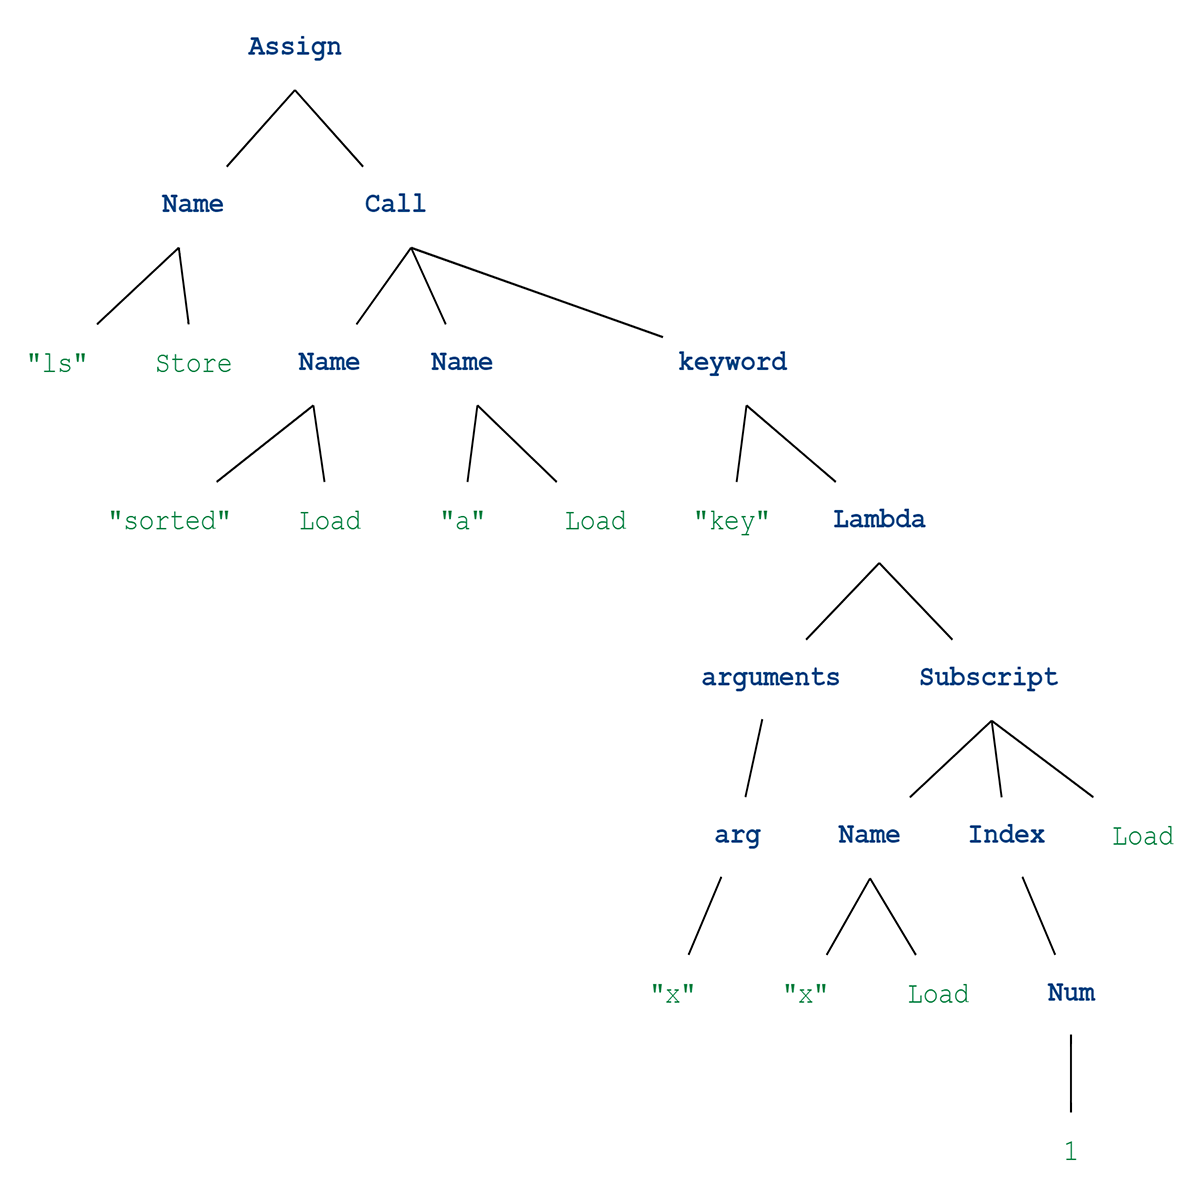
\includegraphics{Figures/ast}
\decoRule
\caption[Abstract Syntax Tree]{Abstract syntax tree of code snippet \code{ls = sorted(a, key=lambda x: x[1])}.}\footnote{Picture is created with Python library \code{showast}\href{https://github.com/hchasestevens/show_ast}}}
\label{fig:ast}
\end{figure}

\section{Semantic structures}
Theory of sentence analysis derives from the idea that the words of a sentence seem to combine into patterns and structures. Each word identified as different in terms of its function in a sentence. According to this function, for each word can be assigned its lexical category or part of speech, like a noun (\code{N}), adjective (\code{A}), or verb (\code{V}). 

This system could be extended to the level of syntactic categories, combining words or other syntactic categories with similar function into phrases. Each phrase is characterized by the properties of the headword that it includes. For example, the headword of the subject of a sentence is a noun, so it is classified as a noun phrase (\code{NP}). A verb is regarded as the head of the sentence predicate, so predicate is classified as a verb phrase (\code{VP}). Rules which describe how lexical categories can be combined into syntactic categories is called rewriting rules. For example, a noun phrase category may be described as the parent of adjective and noun categories, and it may be represented by a rule of the form \code{NP -> A N}. 

A formalization of such rule-based sentence structure system is called a \emph{phrase-based grammar}. Grammar identified by the following constituents:
$V_N$ is a non terminal vocabulary, which contains the lexical and syntactic category labels;
$V_T$ is terminal vocabulary and it contains a set of words.
$P$ identifies the collection of the production rules of the grammar.
To illustrate this concept, I present a short grammar to parse a sentence "`good dogs like cats"' to its syntactic representation. The grammar for this example contains following vocabulary:
\begin{equation}
\begin{split}
V_N = {S, NP, VP, A, N, V}\\
V_T = {cats, dogs, like, nice}
\end{split}
\end{equation}
The production rules for this grammar would be following:
\begin{verbatim}
S => NP VP
NP => A N
NP => N
VP => V NP
N => dogs
N => cats
V => like
A => good
\end{verbatim}
Graphic representation of syntactic tree  of this sentence could be seen in \ref{fig:syntax_tree}.

\begin{figure}
\centering
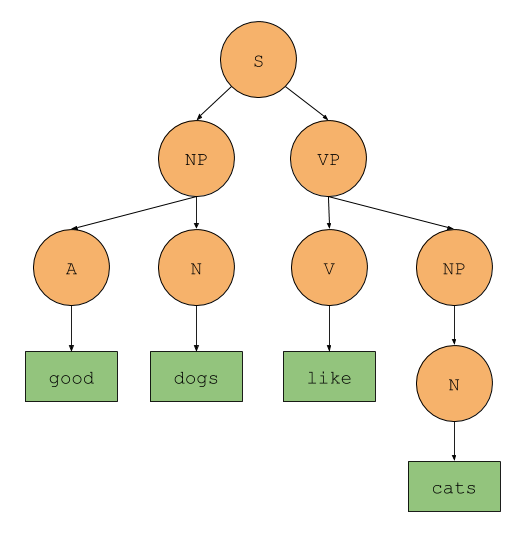
\includegraphics{Figures/syntaxtree}
\decoRule
\caption[Syntax tree]{Example of syntax tree.}
\label{fig:syntax_tree}
\end{figure}

\section{Combinatory-categorial grammar}
% Speech and Language Processing
Phrase-structure grammars analyze the sentence recursively applying rewriting rules, starting from identification of the parts of speech or lexical categories of individual words. This rule governs, how words can be combined into phrases and sentences. Compared with phrase-structure grammars, \emph{combinatory-categorial grammars} do not contain a separate collection of category-combining rules. Lexical categories of words such adjectives and nouns describe the functions that determine how these words can combine with other categories. Each node in combinatory-categorial grammar tree can be translated into lambda calculus, though CCG is a transparent interface between syntax and semantics of a sentence. 

Let's consider an example. Adjective ‘good’ is in a category corresponding to a function that maps from the nouns into the noun phrases. The association of this item with a function looks like that:

\begin{verbatim}
good = NP/N 
\end{verbatim}

$\lambda x.good(x)$\footnote{To make connection of CCG categories with lambda calculus clear, I will complement each example of categorial operations with lines of lambda calculus.}

\code{NP} on the left side of the slash character denotes function return value and \code{N} on the right side denotes function argument. This function could be resolved with forward function application operation, denoted by character \code{>}:

\begin{verbatim}
dogs => N
good dogs => NP/N>N = NP
\end{verbatim}

$\lambda x.good(x)(DOGS)=good(DOGS)$

With backward slash character \code{\textbackslash} right side category denotes function return and left side denotes function argument. Example:

\begin{verbatim}
bird => N
flies => N\textbackslash S
bird flies => N>N\textbackslash S = S
\end{verbatim}

$\lambda x.flies(x)$

$\lambda x.flies(x)(BIRD)=flies(BIRD) $

A verb such as ‘like’ is usually taking two arguments and associated as follows:

\begin{verbatim}
like => (S/NP)\textbackslash N
cats => N
like cats => (S/NP)\textbackslash N>N = S/NP
\end{verbatim}

$\lambda x.\lambda y.like(x, y)$

$\lambda x.\lambda y.like(y, x)(CATS)=\lambda y.like(y, CATS)$

The function \code{(S/NP)\\N} maps \code{N} to a range of functions of form \code{S/NP}.  Character \code{<} denotes backward function application. Final sentence example:

\begin{verbatim}
good dogs => NP
like cats => S/NP
good dogs like cats => NP<S/NP = S
\end{verbatim}

$\lambda y.like(y, CATS)$

$\lambda y.like(y, CATS)(good(DOGS))=like(good(DOGS), CATS)$

% dependency parsing vs constituency parsing

\section{Word embeddings}
The task of language modeling requires the transformation of words and documents into some vector representation. Simple tasks like text classification could be done using naive representations like a bag of words or one hot encoding. However, these approaches could require excessive memory usage to handle large vocabulary and usually do not infer existing semantical connections between words in a language. 

\begin{figure}
\centering
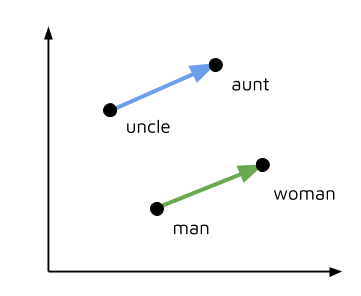
\includegraphics{Figures/word_embeddings}
\decoRule
\caption[Word vectors]{Example of collinearity between two word vectors.}
\label{fig:word_embeddings}
\end{figure}

Methods of \emph{word embeddings} solve both problems, providing dense vectors of real numbers, which represent word positions in $n$-dimensional space. This space represents contextual similarity of the words, thus word embeddings support semantic relations as vector operations. For example, adding vector ‘woman’ to vector ‘uncle’ and subtracting vector ‘man’ will result in vector approximately pointing in the same point as vector ‘aunt’ (see \ref{fig:word_embeddings} for example).

\section{Long-short term memory network}
Model of LSTM network is an extension of the simple recurrent network. It can store values in the hidden layer for a short or long period of time because it uses no activation function within its recurrent components. This makes able to backpropagate error gradient through long sequences of data without gradient vanishing or gradient exploding.

\begin{figure}
\centering
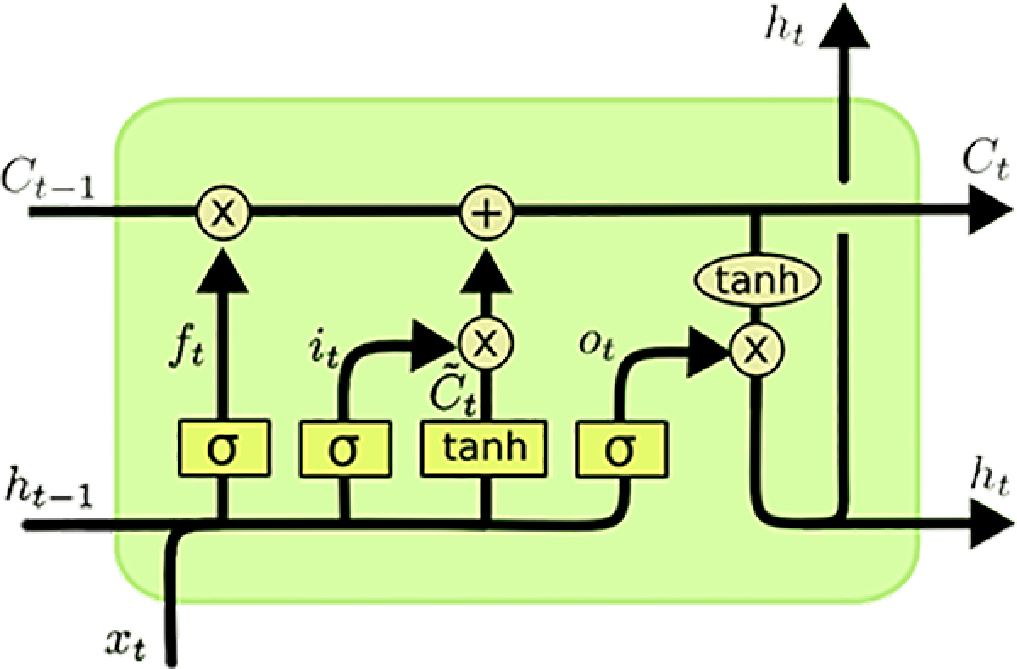
\includegraphics{Figures/lstm}
\decoRule
\caption[Long-short term memory]{Long-short term memory network achitecture \parencite{lstm-picture}.}
\label{fig:word_embeddings}
\end{figure}

Forget gate:
\begin{equation}
f_t = \sigma(W_f\cdot[h_{t-1},x_t] + b_f)
\label{lstm:ft}
\end{equation} 

Input gate and new memory state ($\circ$ denotes entrywise product):
\begin{equation}
i_t=\sigma(W_i\cdot[h_{t-1}, x_t]+b_i)
\label{lstm:input}
\end{equation} 

\begin{equation}
\widetilde{C}_t = tanh(W_c\cdot[h_{t-1}, x_t]+b_C)
\label{lstm:c1}
\end{equation} 

\begin{equation}
C_t = f_t\circ C_{t-1}+i_t\circ\widetilde{C}_t
\label{lstm:c2}
\end{equation} 

Gate for new hidden state:
\begin{equation}
o_t=\sigma(W_o[h_{t-1},x_t]+b_o)
\label{lstm:o}
\end{equation} 

\begin{equation}
h_t=o_t\circ tanh(C_t)
\label{lstm:h}
\end{equation}

\section{Sequence to sequence machine translation with attention}
% http://phontron.com/class/mtandseq2seq2017/mt-spring2017.chapter8.pdf
The task of machine translation can be formalized as mapping of a sequence of words in a source language to a sequence of words in a target language. This task can be solved with an \emph{encoder-decoder} model, which consists of two recurrent neural networks. The first RNN consumes input sequence step by step and encodes it into so-called thought vector. After encoding, the second RNN uses thought vector as its initial hidden state and decodes output sentence word by word.  Each word from decoder output is used as input for the next decoding step until the model outputs the end-of-sentence token. 

Theoretically, a sufficiently large encoder-decoder model should be able to perform machine translation perfectly. However, to encode all words and dependencies between them in the arbitrary-length sentences the thought vector should have enormous length. It would require massive computational resources to train and use such architecture and though this approach is ineffective.

This problem can be solved with attention technique. Its basic idea is to replace single vector representation of input sentence with references to representations of different words in it. On the encoding step, each word representation $h_e(t)$ stored as a column of matrix $H_e$. During the decoding step, hidden state of decoder network calculated as follows:

% пояснити
\begin{equation}
h_d(t) = enc([embed(w(t));c(t-1)], h_d(t-1))
\label{attn:hd}
\end{equation}

\begin{figure}
\centering
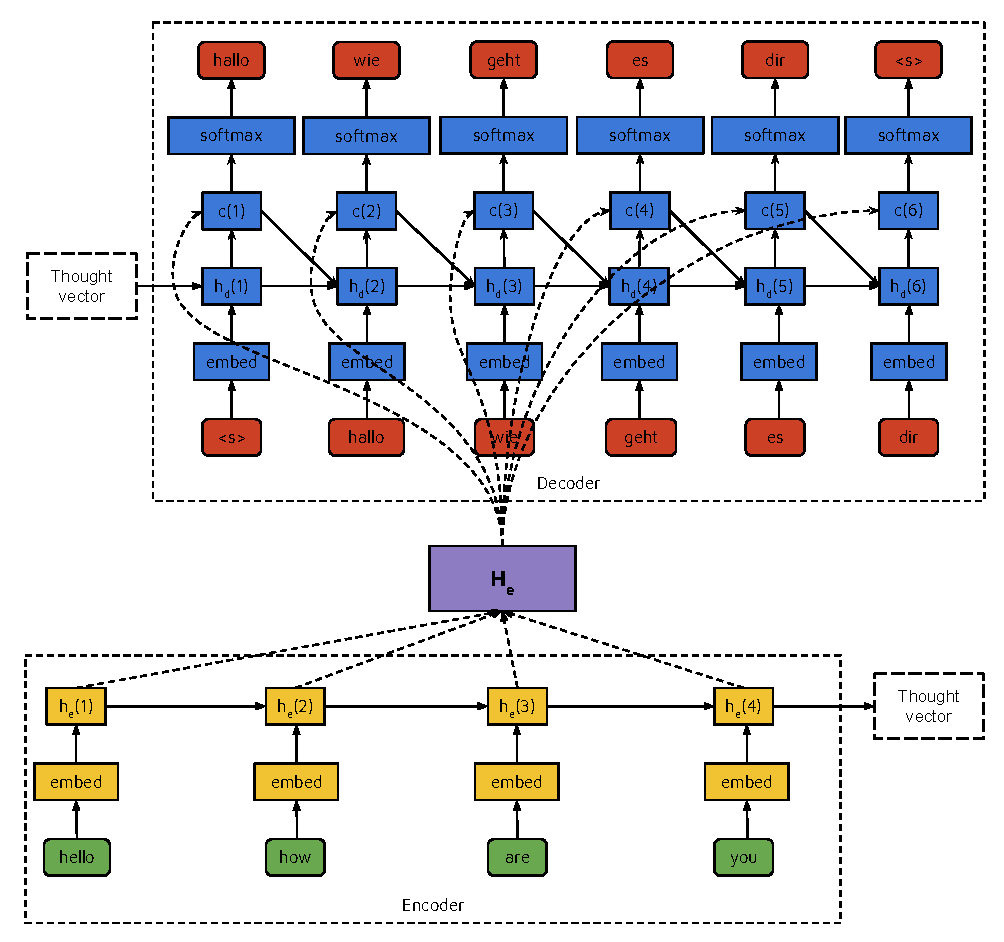
\includegraphics{Figures/seq2seq}
\decoRule
\caption[Sequence to sequence model]{Sequence to sequence with attention model.}
\label{fig:seq2seq}
\end{figure}

Elements of attention vector calculated with arbitrary attention score function (for example, vector product) for each pair of decoder and encoder representations:
\begin{equation}
\alpha_j(t) = attnscore(h_e(j), h_d(t))
\label{attn:alpha}
\end{equation}

\begin{equation}
\alpha_j(t) = softmax(\alpha_j(t))
\label{attn:alpha2}
\end{equation}

Then context vector calculated as a weighted sum of encoder representations:
\begin{equation}
	c(t) = H_e\cdot\alpha(t)
	\label{attn:c}
\end{equation}

\begin{equation}
	P(t) = softmax(W_{hs}\cdot[h_d(t);c(t)])
\label{attn:P}
\end{equation}

This way each decoder step can use information from arbitrary part of encoded sequence. Input sentence representation should not be limited to fixed length though vector and though it can model natural language with adequate model size. An architecture of sequence to sequence model with attention can be seen at the \ref{fig:seq2seq}.

\section{Recursive neural networks}
% reflectes inductive bias
The architecture of recurrent neural network reflects domain knowledge about conditional probability of target variable with previous values in a sequence. Representation of natural language can also be modeled as a plain sequence of words. However, this approach ignores domain knowledge about the syntactic structure of a text. A syntactic tree contains important information about relations between individual terms and thus should not be omitted in the task of natural language meaning representation.
\begin{figure}
\centering
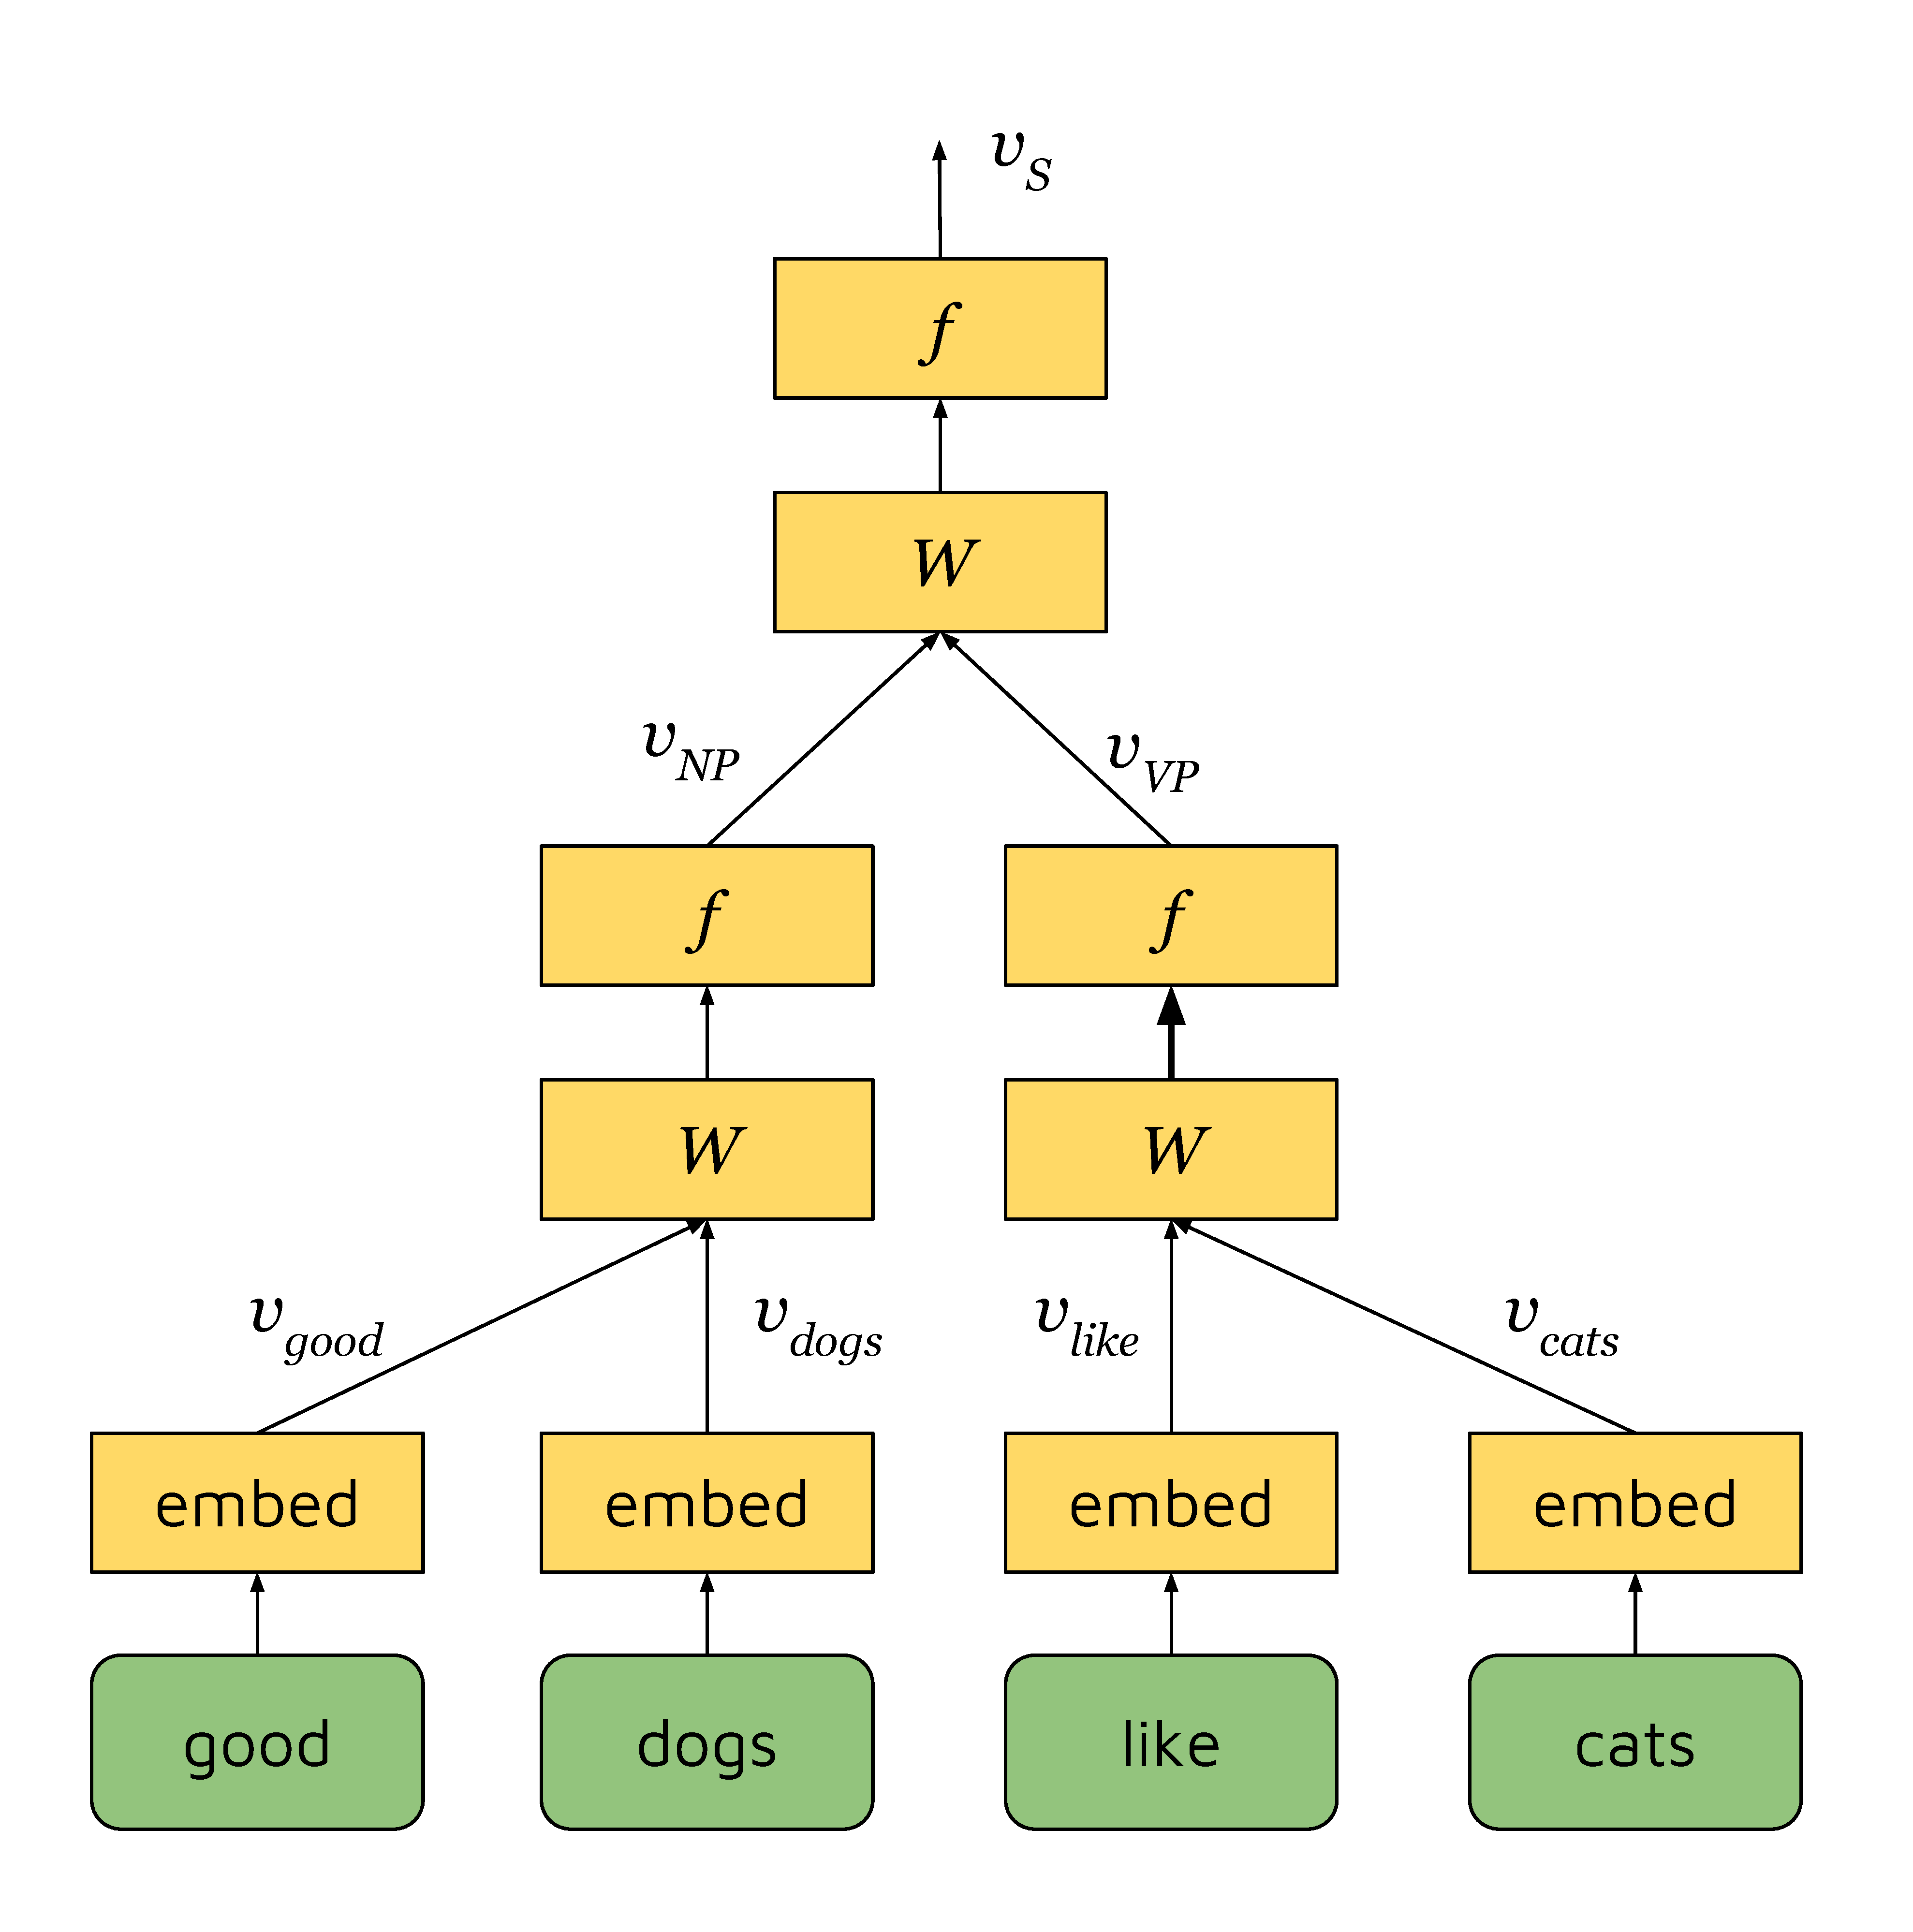
\includegraphics{Figures/rvnn}
\decoRule
\caption[RvNN flow]{Examle of recursive neural network flow.}
\label{fig:rvnn}
\end{figure}
Topological structures with variable length could be modeled by neural networks recursively applying the same set of weight to each node. To model syntactic tree, each word is represented by corresponding embedding vector and then parent vectors are computed using a bottom-up approach with composition functions. For example, representation of the syntactic tree of sentence good dog like cats could be modeled the following way:
\begin{equation}
\begin{split}
v_{NP} = f(W\cdot[v_{good}, v_{dog}])\\
v_{VP} = f(W\cdot[v_{like}, v_{cats}])\\
v_S = f(W\cdot[v_{NP}, v_{VP}])
\label{rvnn:example}
\end{split}
\end{equation}
where $f$ is any differentiable non-linearity like $tanh$ or $relu$. The example of semantic tree parsing with recursive network presented at \ref{fig:rvnn}. 

\section{Pointer networks}

\chapter{Model} 
\label{Chapter4}

\section{Code generation problem}
Given a natural language description $x$ our task is to infer the Python code $y$ based on the intent of the $x$. Python code $y$ can be deterministically converted to an AST $\tau$ and vice-versa, though in this work a source code $y$ and its abstract syntax tree $\tau$ are considered equivalent. A probabilistic grammar model of generating an abstract syntax tree $\tau$ given description $x$ is defined as $P(\tau|x)$. The best corresponding syntax tree $\tau$ is defined as
\begin{equation}
\hat{\tau}=\underset{\tau}{\operatorname{argmax}}\: p(\tau|x)
\label{eqn:main_problem}
\end{equation}
Probability from Eq. \ref{eqn:main_problem} is modeled with neural model with a set of weights $\theta$. To learn values of $\theta$ we used a set of training examples, which consist of tuples $(\tau^{(x)}, x)$. The parameters of the model are learned by maximizing the conditional log-probabilities for the training set:
\begin{equation}
\theta=\underset{\theta}{\operatorname{argmax}} \sum_{\tau^{(x)}, x} log \: p(\tau^{(x)}|x; \theta)
\label{eqn:mle}
\end{equation}

\section{Abstract syntax tree generation} \label{ast_gen}
The output of decoder is an abstract syntax tree which consist of terminal and non-terminal nodes. As suggested in work of \cite{Yin2017}, we factorized the generation process of AST into sequential application of actions of two types:
\begin{itemize}
	\item \code{ApplyRule[r]} corresponds to non-terminal nodes. It applies a production rule \code{r} to the current derivation tree.
	\item \code{GenToken[v]} corresponds to terminal nodes. It finishes the node by appending a token \code{v}.
\end{itemize}

Let us consider as example the AST from \cref{fig:ast}. Its generation consist of the following actions:

\begin{codelist}{AST production sequence.}
\begin{verbnobox}[\verbarg]
ApplyRule[root => (stmt*)]
    ApplyRule[stmt => (Assign)]
        ApplyRule[Assign => (expr*{targets}), (expr{value})]
            ApplyRule[expr* => (expr)]
                ApplyRule[expr => (Name)]
                    ApplyRule[Name -> (str{id})]
                        GenToken["ls"]
                        GenToken["<eos>"]
            ApplyRule[expr => (Call)]
                ApplyRule[Call => (expr{func}), (expr*{args}), (keyword*{keywords})]
                    ApplyRule[expr => (Name)]
                        ApplyRule[Name -> (str{id})]
                            GenToken["sorted"]
                            GenToken["<eos>"]
                    ApplyRule[expr* => expr]
                        ApplyRule[expr => (Name)]
                            ApplyRule[Name => (str{id})]
                                GenToken["a"]
                                GenToken["<eos>"]
                    ApplyRule[keyword* => keyword]
                        ApplyRule[keyword => (str{arg}), (expr{value})]
                            GenToken["key"]
                            GenToken["<eos>"]
                            ApplyRule[expr => (Lambda)]
...
ApplyRule[Lambda => (arguments args), (expr body)]
    ApplyRule[arguments => (arg* args)]
        ApplyRule[arg* => arg]
            ApplyRule[arg => (str{arg})]
                GenToken["x"]
                GenToken["<eos>"]
    ApplyRule[expr => Subscript]
        ApplyRule[Subscript => (expr{value}), (slice{slice})]
            ApplyRule[expr => (Name)]
                ApplyRule[Name => (str{id})]
                    GenToken["x"]
                    GenToken["<eos>"]
            ApplyRule[slice => (Index)]
                ApplyRule[Index => (expr{value})]
                    ApplyRule[expr => (Num)]
                        ApplyRule[Num => (int{n})]
                            GenToken["1"]
                            GenToken["<eos>"]
\end{verbnobox}
\label{code:ast_production}
\end{codelist}

Under this grammar model, the probability of generating an AST $\tau$ is factorized as:
\begin{equation}
p(\tau|x) = \prod^{n}_{t=1} p(a^{(t)}|x, a^{(<t)})
\label{eqn:tree_probability}
\end{equation}
where $a^{t}$ is an action taken at the time step $t$ and $a_{<t}$ is the sequence of actions before $t$. 

For each time step $t$ the model selects the next action with a maximum probability --- \code{ApplyRule} to grow the tree or \code{GenToken} to fill values in terminal nodes. We must notice, that this model have one important flaw. List nodes like a \code{expr*} can not be expanded to an arbitrary number of children. Each number of children require separate rule in the grammar, like \code{expr* => (expr), (expr)}, \code{expr* => (expr), (expr), (expr)} etc. Therefore this model will require huge vocabulary to cover all possible production rules in dataset with arbitrary length functions. We proposed our solution to this issue in \cref{improve}.

\subsection{ApplyRule actions}
At any generation moment a tree $\tau$ contains a single frontier node (for time step $t$ it is $n_{f_t}$). An action \code{ApplyRule} expands frontier node in depth-first, left-to-right traversal of the tree. A production rule $r$ expands $n_{f_t}$ by appending all child nodes specified by the selected production. For example, in listing \ref{code:ast_production} in step 10 rule for node \code{Call} extends this node with three new nodes: \code{expr\{func\}}, \code{expr*\{args\}}, \code{keyword*\{keywords\}}. 

When $n_{f_t}$ is a terminal node, which can not be expanded further, the next action must be \code{GenToken}.

\textbf{Unary closures}. Sometimes, generating an AST requires applying a chain of unary productions. For example, in listing \ref{code:ast_production} in steps 4-6 it takes three time step to generate target for \code{Assign} statement:

\begin{verbatim}
ApplyRule[expr* => (expr)]
    ApplyRule[expr => (Name)]
        ApplyRule[Name -> (str{id})]
\end{verbatim}

Such a formal redundancy allows to have smaller production rule grammar but would increase a sequence length. Thus, they can be replaced with one action by taking the closure of the chain of unary productions:

\begin{verbatim}
ApplyRule[expr* => (str{id})]
\end{verbatim}

Model was tested both with and without unary closures.

\subsection{GenToken actions} \label{gentoken}
If a tree has reached a leaf and $n_{f_t}$ is a terminal node, the \code{GenToken} actions is used to fill this node. Each token generation ends with special end-of-string token \code{"<eos>"}. This way complex tokens like the function name \code{sortBySecondIndex} can be split on parts \code{['sort', 'By', 'Second', 'Index']}, thus reduce the token vocabulary and allow a complex rare token to be constructed from its constituents. After the end-of-string token generation model proceeds to the next frontier node.

The vocabulary of predefined token values can be inferred from the dataset. However, it is clear that this vocabulary will not cover all possible tokens for any environment. To cope with this problem, values can be copied directly from the input sequence. Therefore, it allows the model to use literals and names from a code description.

\section{Action probabilities}
Probabilities in \cref{eqn:tree_probability} are estimated by a neural attentional encoder-decoder model. Both encoder and decoder informational flow is structured by syntactic trees. 

\subsection{Encoder}
The main architectural novelty in this work is a Tree-LSTM encoder. Details about its input structures and implementation described below.

Input NL description $x$ consist of two parts. The first is a sequence of length $n$ of word vectors $\{w^{(t)}\}^n_{t=1}$. The second is a syntax tree which consists of $m$ nodes $\{\eta^{(t)}\}^m_{t=1}$, where $m\geq n$. Details about the description tree parsing can be found in \cref{preprocessing}. For all $t \leq n$, each tree node $\eta^{(t)}$ has a corresponding input vector from a word sequences $w^{(t)}$. For $t > n$, an input vector for $\eta^{(t)}$ is padding-vector. Each tree node $\eta^{(t)}$ has a set of children nodes $ch(\eta^{(t)})=\{\eta_{i}\}^k_{i=1}$. Therefore a single input element $x^{(t)}$ can be defined as a tuple $(\eta^{(t)}, w^{(t)}, ch(\eta^{(t)}))$:

\begin{equation}
 x^{(t)} =
  \begin{cases}
    (\eta^{(t)}, w^{(t)}, ch(\eta^{(t)}))  & \quad \text{if } t\leq n\\
    (\eta^{(t)}, w_{pad}, ch(\eta^{(t)}))  & \quad \text{if } t > n
  \end{cases}
\label{eq:enc_input}
\end{equation}

To encode this structures we used Tree-LSTM from \cite{Tai2015}\footnote{We used pytorch implementation from \href{https://github.com/dasguptar/treelstm.pytorch}{https://github.com/dasguptar/treelstm.pytorch}}. Similary to SRvN, described in \cref{sec:rvnn}, this model starts from tree leaves, and recursively computes a node embedding $h^{(t)}$ for each $x^{(t)}$ using values of a memory cell $\{c_i\}^{k}_{i=1} = memory(ch(\eta^{(t)}))$ and previous  embeddings $\{h_i\}^{k}_{i=1} = hidden(ch(\eta^{(t)}))$ from children nodes:

\begin{equation}
\begin{gathered}
    \hat{h} = \sum^{k}_{i=1}h_i \\
    
    i^{(t)} = \sigma(W_i\cdot[\hat{h}, w^{(t)}]+b_i) \\
    
    u^{(t)} = tanh(W_u\cdot[\hat{h}, w^{(t)}]+b_u) \\
    
    f^{(t)}_i = \sigma(W_{f}\cdot [h_i, w^{(t)}] + b_f) \\
    
    c^{(t)} = i^{(t)} \circ u^{(t)} + \sum_{i=1}^{k} f^{(t)}_i \circ c_i \\
    
    o^{(t)} = \sigma(W_o\cdot[\hat{h}, w^{(t)}]+b_o) \\
    
    h^{(t)} = o^{(t)} \circ tanh(c^{(t)})

\end{gathered}
\label{eq:tree_lstm}
\end{equation}

\subsection{Decoder}
The decoder is a RNN which sequentially generates an AST model as defined in \cref{eqn:tree_probability}. Each production action naturally grounds to a step in the decoder. This way, the sequence of production rules from listing \ref{code:ast_production} can be interpreted as unrolling RNN time steps with some additional connections from parent action steps.

We used implementation of decoder from \cite{Yin2017}. It is vanilla LSTM with additional connections which reflect the topological structure of the code syntax. For each decoding step, input vector is concatenation of a frontier node embedding $n^{(t)}$, a previous action embedding $a^{(t-1)}$ and a parent feeding $p^{(t)}$. The parent feeding is a concatenation of a decoder hidden state from parent step $h_{dp}^{(t)}$ and a parent rule embedding $r_p^{(t)}$. Consider as example step 9 in listing \ref{code:ast_production}: 
    
\begin{verbatim}
ApplyRule[Assign => (expr*{targets}), (expr{value})]
    ...............
                GetToken["<eos>"]
    ApplyRule[expr => (Call)]
\end{verbatim}

It has a frontier node \code{expr}, a previous action \code{GetToken["<eos>"]} and a parent rule \code{Assign => (expr*\{targets\}), (expr\{value\})}. Corresponding vectors for the node, rule and token stored as column vectors in matrices $W_n$, $W_r$, $W_v$.

Additionally, a decoder input contains attention and attention over history context vectors. The context vectors are calculated as described in \cref{attention}. Attention over history uses vectors from a previous decoder output:

\begin{equation}
    \phi_h^{(t)} = H_d\cdot\alpha_h^{(t)}
\end{equation}

Given all described above input values and a previous decoder embedding $h_d^{(t-1)}$, the next decoding step is calculated as following:

\begin{equation}
    h_d^{(t)}=f_{lstm}([a^{(t-1)}, n^{(t)}, p^{(t)}, \phi^{(t-1)}, \phi_h^{(t-1)}], h_d^{(t-1)})
\end{equation}

\subsection{Calculating probabilities}
In this section we explained how action probabilities from  \cref{eqn:tree_probability} are calculated from a decoder embeddings $h^{(t)}$.

\textbf{ApplyRule}. The probability of applying a rule $r$ as the current action $a^{(t)}$ is given by a softmax:

\begin{equation}
\begin{gathered}
    h^{(t)}_r = tanh(W _{r1}\cdot h^{(t)} + b_{r1}) \\
    P_r = softmax(W_r\cdot h^{(t)}_r  + b_r) \\
    p(a^{(t)} = ApplyRule[r]|x,a^{(<t)}) = P_r\cdot e(r)
\end{gathered}
\label{eqn:apply_rule}
\end{equation}

where $e(r)$ is one-hot embedding for rule $r$.

\textbf{GenToken}. As described in \cref{gentoken}, a token $v$ can be generated from a predefined vocabulary or copied from the input. Therefore probability of an action to be $GenToken[v]$ is defined as a marginal probability:
    
\begin{equation}
\begin{gathered}
    p(a^{(t)} = GenToken[v]|x,a^{(<t)}) = p(gen|x, a^{(<t)}) p(v|gen, x, a^{(<t)}) + \\
    p(copy|x, a^{(<t)}) p(v|copy, x, a^{(<t)})
\end{gathered}
\end{equation}

\begin{equation}
    p(gen|\cdot), p(copy|\cdot) = softmax(W_s\cdot h^{(t)} + b_s)
\end{equation}

Probability of selection of a token $v$ from the vocabulary is calculated similarly to \cref{eqn:apply_rule}. The difference is that the decoder embedding is concatenated with a context vector $\phi^{(t)}$:

\begin{equation}
\begin{gathered}
    h^{(t)}_v = tanh(W _{v1}\cdot [h^{(t)}, \phi^{(t)}] + b_{v1}) \\
    P_v = softmax(W_v\cdot h^{(t)}_v  + b_v) \\
    p(v|gen, x, a^{(<t)}) = P_v\cdot e(v)
\end{gathered}
\label{eq:vocab_gen}
\end{equation}

To model the copy probability we used a pointer network \parencite{Vinyals2015} described in the \cref{pointer}. The same as in \cref{eq:vocab_gen}, we used decoder embedding concatenated with the context vector:

\begin{equation}
\begin{gathered}
    P_c = f_{pointer}(H_e, [h^{(t)}, \phi^{(t)}]) \\
    p(v|copy, x, a^{(<t)}) = P_c \cdot e(v)
\end{gathered}
\end{equation}

Usage of concatenated vector $[h^{(t)}, \phi^{(t)}]$ for token generation probability calculation is reasonable since tokens are likely to occur in the input sequence, thus context vector might store important information.

\section{Training and Inference}

Values for all weights and biases were inferred from training examples, as described in \cref{eqn:mle}. Each AST $\tau$ from a training set was transformed into a sequence of ground truth actions. The next decoder input is selected from ground truth sequence (the teacher forcing, described in  \cref{seq2seq}). The model is optimized by maximizing the log-likelihood of the ground truth actions sequence. Optimization was performed by the method of error back-propagation using ADAM \parencite{Kingma2014} algorithm. At inference time, given an NL description, we used beam search, described in \cref{beam} to approximate the best AST $\hat{y}$ in \cref{eqn:main_problem}.



 
\chapter{Experiments} \label{Chapter5} 


\section{Datasets preprocessing} \label{preprocessing}
% A* CCG Parsing with a Supertag and Dependency Factored Model
% https://nlp.stanford.edu/pubs/glove.pdf 
% dependency parsing https://web.stanford.edu/~jurafsky/slp3/
% https://nlp.stanford.edu/software/stanford-dependencies.shtml
% CCG - mark steedman
% Danqi Chen and Christopher D Manning. 2014. A Fast and Accurate Dependency Parser using Neural Networks. Proceedings of EMNLP 2014
% Jonathan Berant, Andrew Chou, Roy Frostig, Percy Liang. Semantic Parsing on Freebase from Question-Answer Pairs. Empirical Methods in Natural Language Processing (EMNLP), 2013.

\section{Evaluation metrics}
BLEU
Accuracy
Error

rewrite: These two metrics are not ideal: accuracy only measures exact match and thus lacks the ability to give credit to semantically correct code that is different from the reference, while it is not clear whether BLEU provides an appropriate proxy for measuring semantics in the code generation task. A more
intriguing metric would be directly measuring semantic/functional code equivalence, for which we present a pilot study
at the end of this section (cf. Error Analysis). We leave exploring more sophisticated metrics (e.g. based on static code
analysis) as future work.

\section{Results}

Describe previous results. Could be used results from \cite{Yin2017} and \cite{Barone2017}.
Dropout



% Chapter Template

\chapter{Conclusion} % Main chapter title

\label{Chapter6} % Change X to a consecutive number; for referencing this chapter elsewhere, use \ref{ChapterX}
 

\appendix 

% Appendix A

\chapter{Frequently Asked Questions} % Main appendix title

\label{AppendixA} % For referencing this appendix elsewhere, use \ref{AppendixA}

\section{How do I change the colors of links?}

The color of links can be changed to your liking using:

{\small\verb!\hypersetup{urlcolor=red}!}, or

{\small\verb!\hypersetup{citecolor=green}!}, or

{\small\verb!\hypersetup{allcolor=blue}!}.

\noindent If you want to completely hide the links, you can use:

{\small\verb!\hypersetup{allcolors=.}!}, or even better: 

{\small\verb!\hypersetup{hidelinks}!}.

\noindent If you want to have obvious links in the PDF but not the printed text, use:

{\small\verb!\hypersetup{colorlinks=false}!}.

%\include{Appendices/AppendixB}
%\include{Appendices/AppendixC}
\printbibliography[heading=bibintoc]
\end{document}  
